% Copyright (c) 2010 Jérémie DECOCK (http://www.jdhp.org)

\documentclass[pdftex,a4paper,11pt]{article} 
\usepackage[utf8]{inputenc}
\usepackage[frenchb]{babel}
\usepackage[pdftex]{graphicx}
\usepackage{amsmath}
\usepackage{subfigure}
\usepackage{hyperref}

\hypersetup{
	pdftoolbar=true,                    % show Acrobat’s toolbar ?
	pdfmenubar=true,                    % show Acrobat’s menu ?
	pdffitwindow=true,                  % page fit to window when opened
	pdftitle={Pyarm},                   % title
	pdfauthor={Jérémie DECOCK},         % author
	pdfsubject={Pyarm},                 % subject of the document
	pdfnewwindow=true,                  % links in new window
	pdfkeywords={Pyarm},                % list of keywords
	colorlinks=true,                    % false: boxed links; true: colored links
	linkcolor=black,                    % color of internal links
	citecolor=black,                    % color of links to bibliography
	filecolor=black,                    % color of file links
	urlcolor=black                      % color of external links
}

\begin{document}

\title{Pyarm}
\author{
	Jérémie \bsc{Decock}
}
\date{\today{}}

\maketitle

%%%%%%%%%%%%%%%%%%%%%%%%%%%%%%%%%%%%%%%%%%%%%%%%%%%%%%%%%%%%%%%%%%%%%%%%%%%%%%%%

\section{Présentation des modèles}

\subsection{Présentation}

\begin{center}
        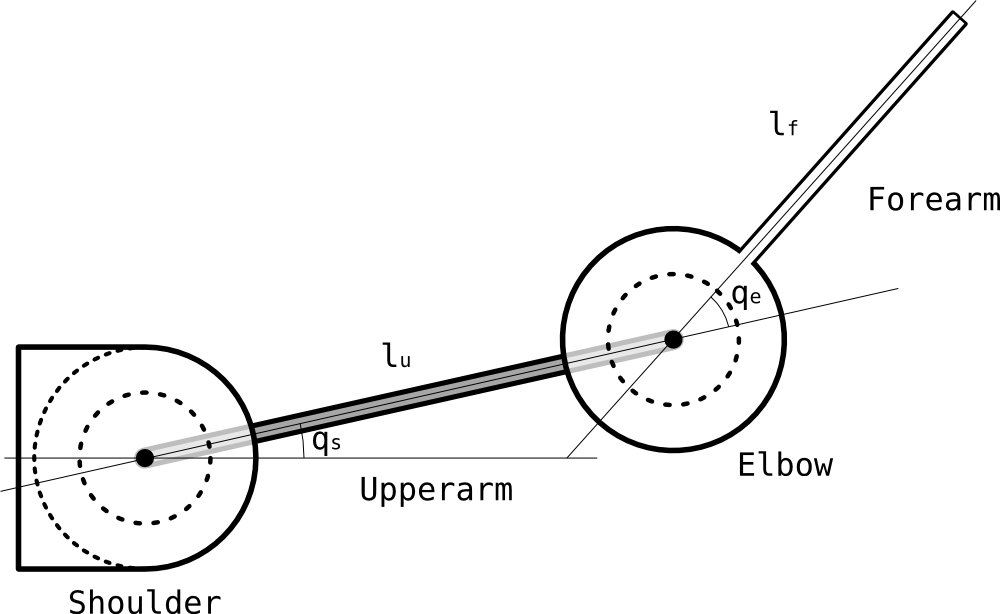
\includegraphics[width=.40\linewidth]{fig/arm}
\end{center}

\begin{itemize}
    \item Bras 2D
    \item Plan horizontal (Mitrovic, Weiwei) ou vertical (Kambara)
    \item 2 articulations (épaule et coude)
    \item 6 muscles~:
    \begin{enumerate}
        \item fléchisseur de l'épaule
        \item extenseur de l'épaule
        \item fléchisseur du coude
        \item extenseur du coude
        \item fléchisseur
        \item extenseur
    \end{enumerate}
\end{itemize}

\subsection{Les modèles étudiés}
Trois modèles ont été étudiés~:
\begin{itemize}
    \item Katayama / Mitrovic
    \item Kambara
    \item Brown / Weiwei
\end{itemize}

\subsection{Simulateur Pyarm}

\begin{itemize}
    \item Codé en Python
    \item Implémente les 3 modèles
\end{itemize}

%\begin{center}
%    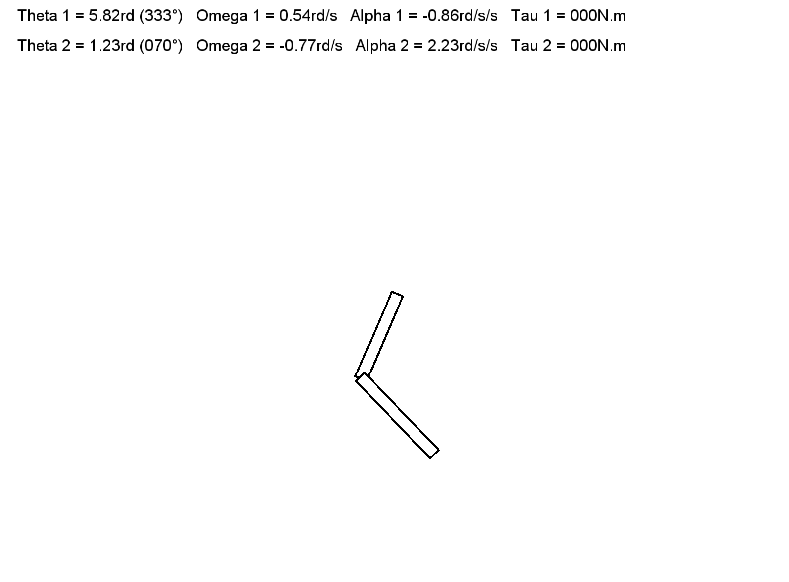
\includegraphics[width=.40\linewidth]{fig/pyarm1}
%\end{center}
\begin{figure}
    \centering
    \subfigure{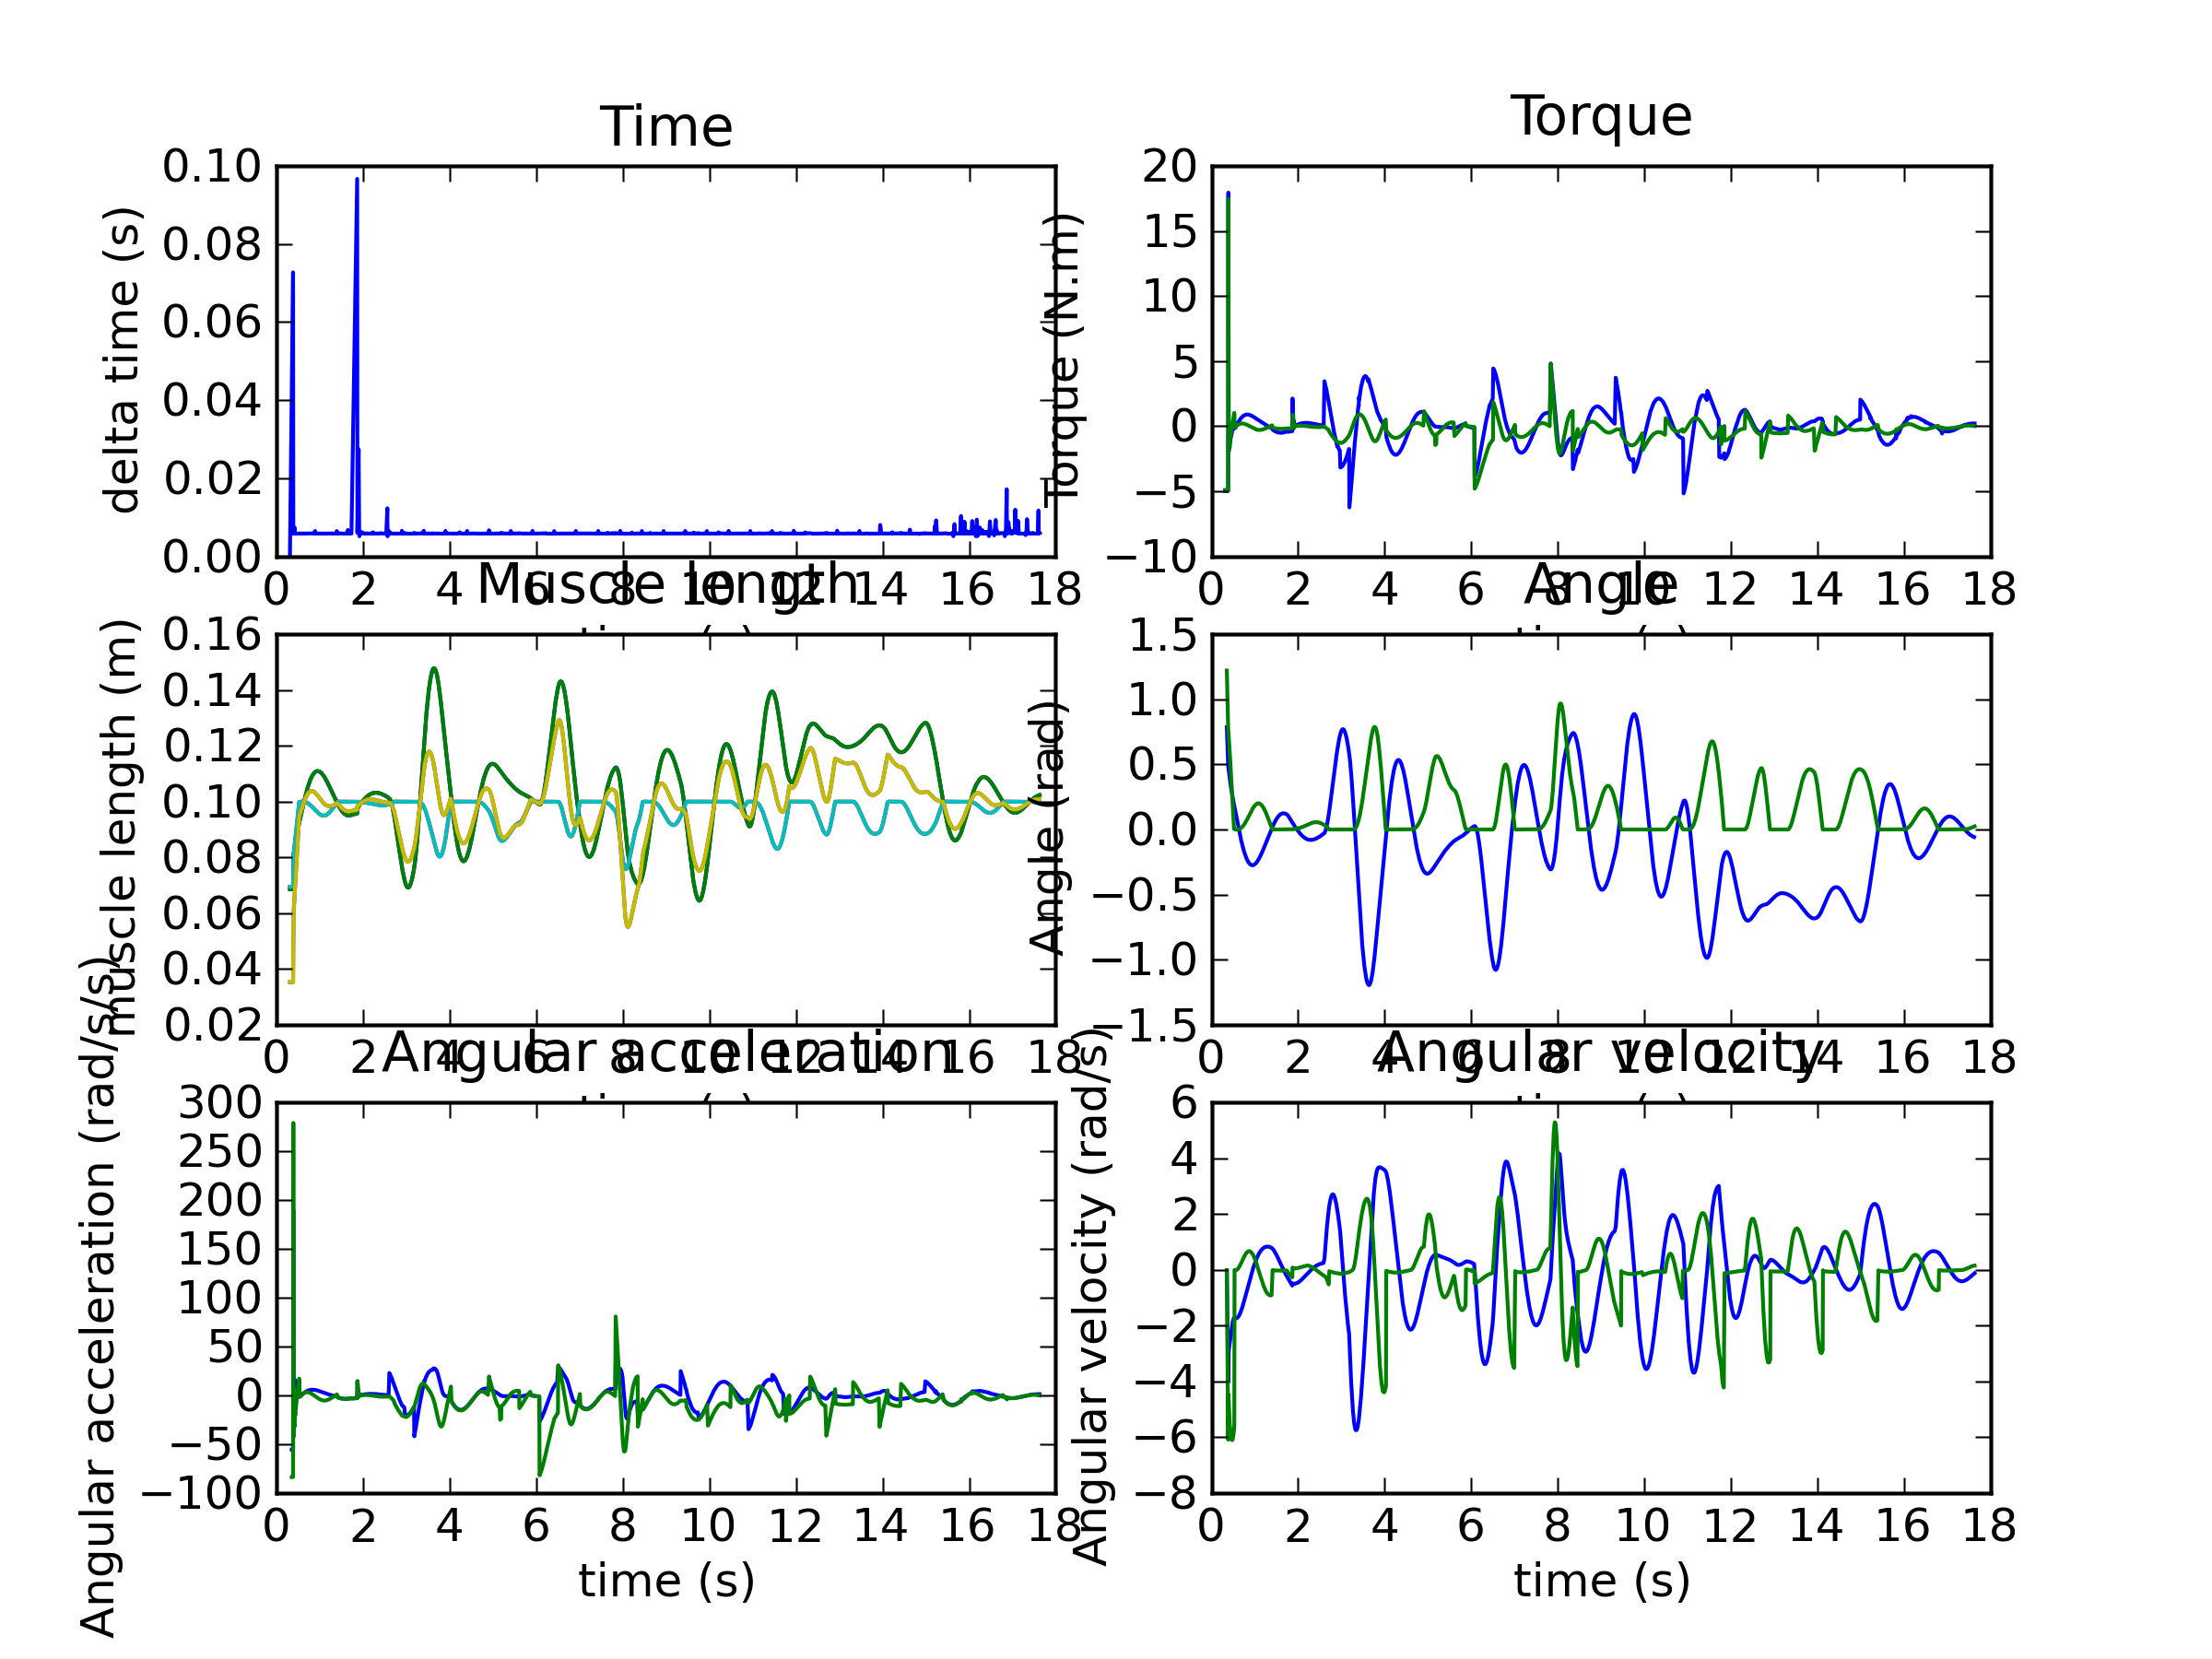
\includegraphics[width=.50\linewidth]{fig/pyarm2}}~~~
    \subfigure{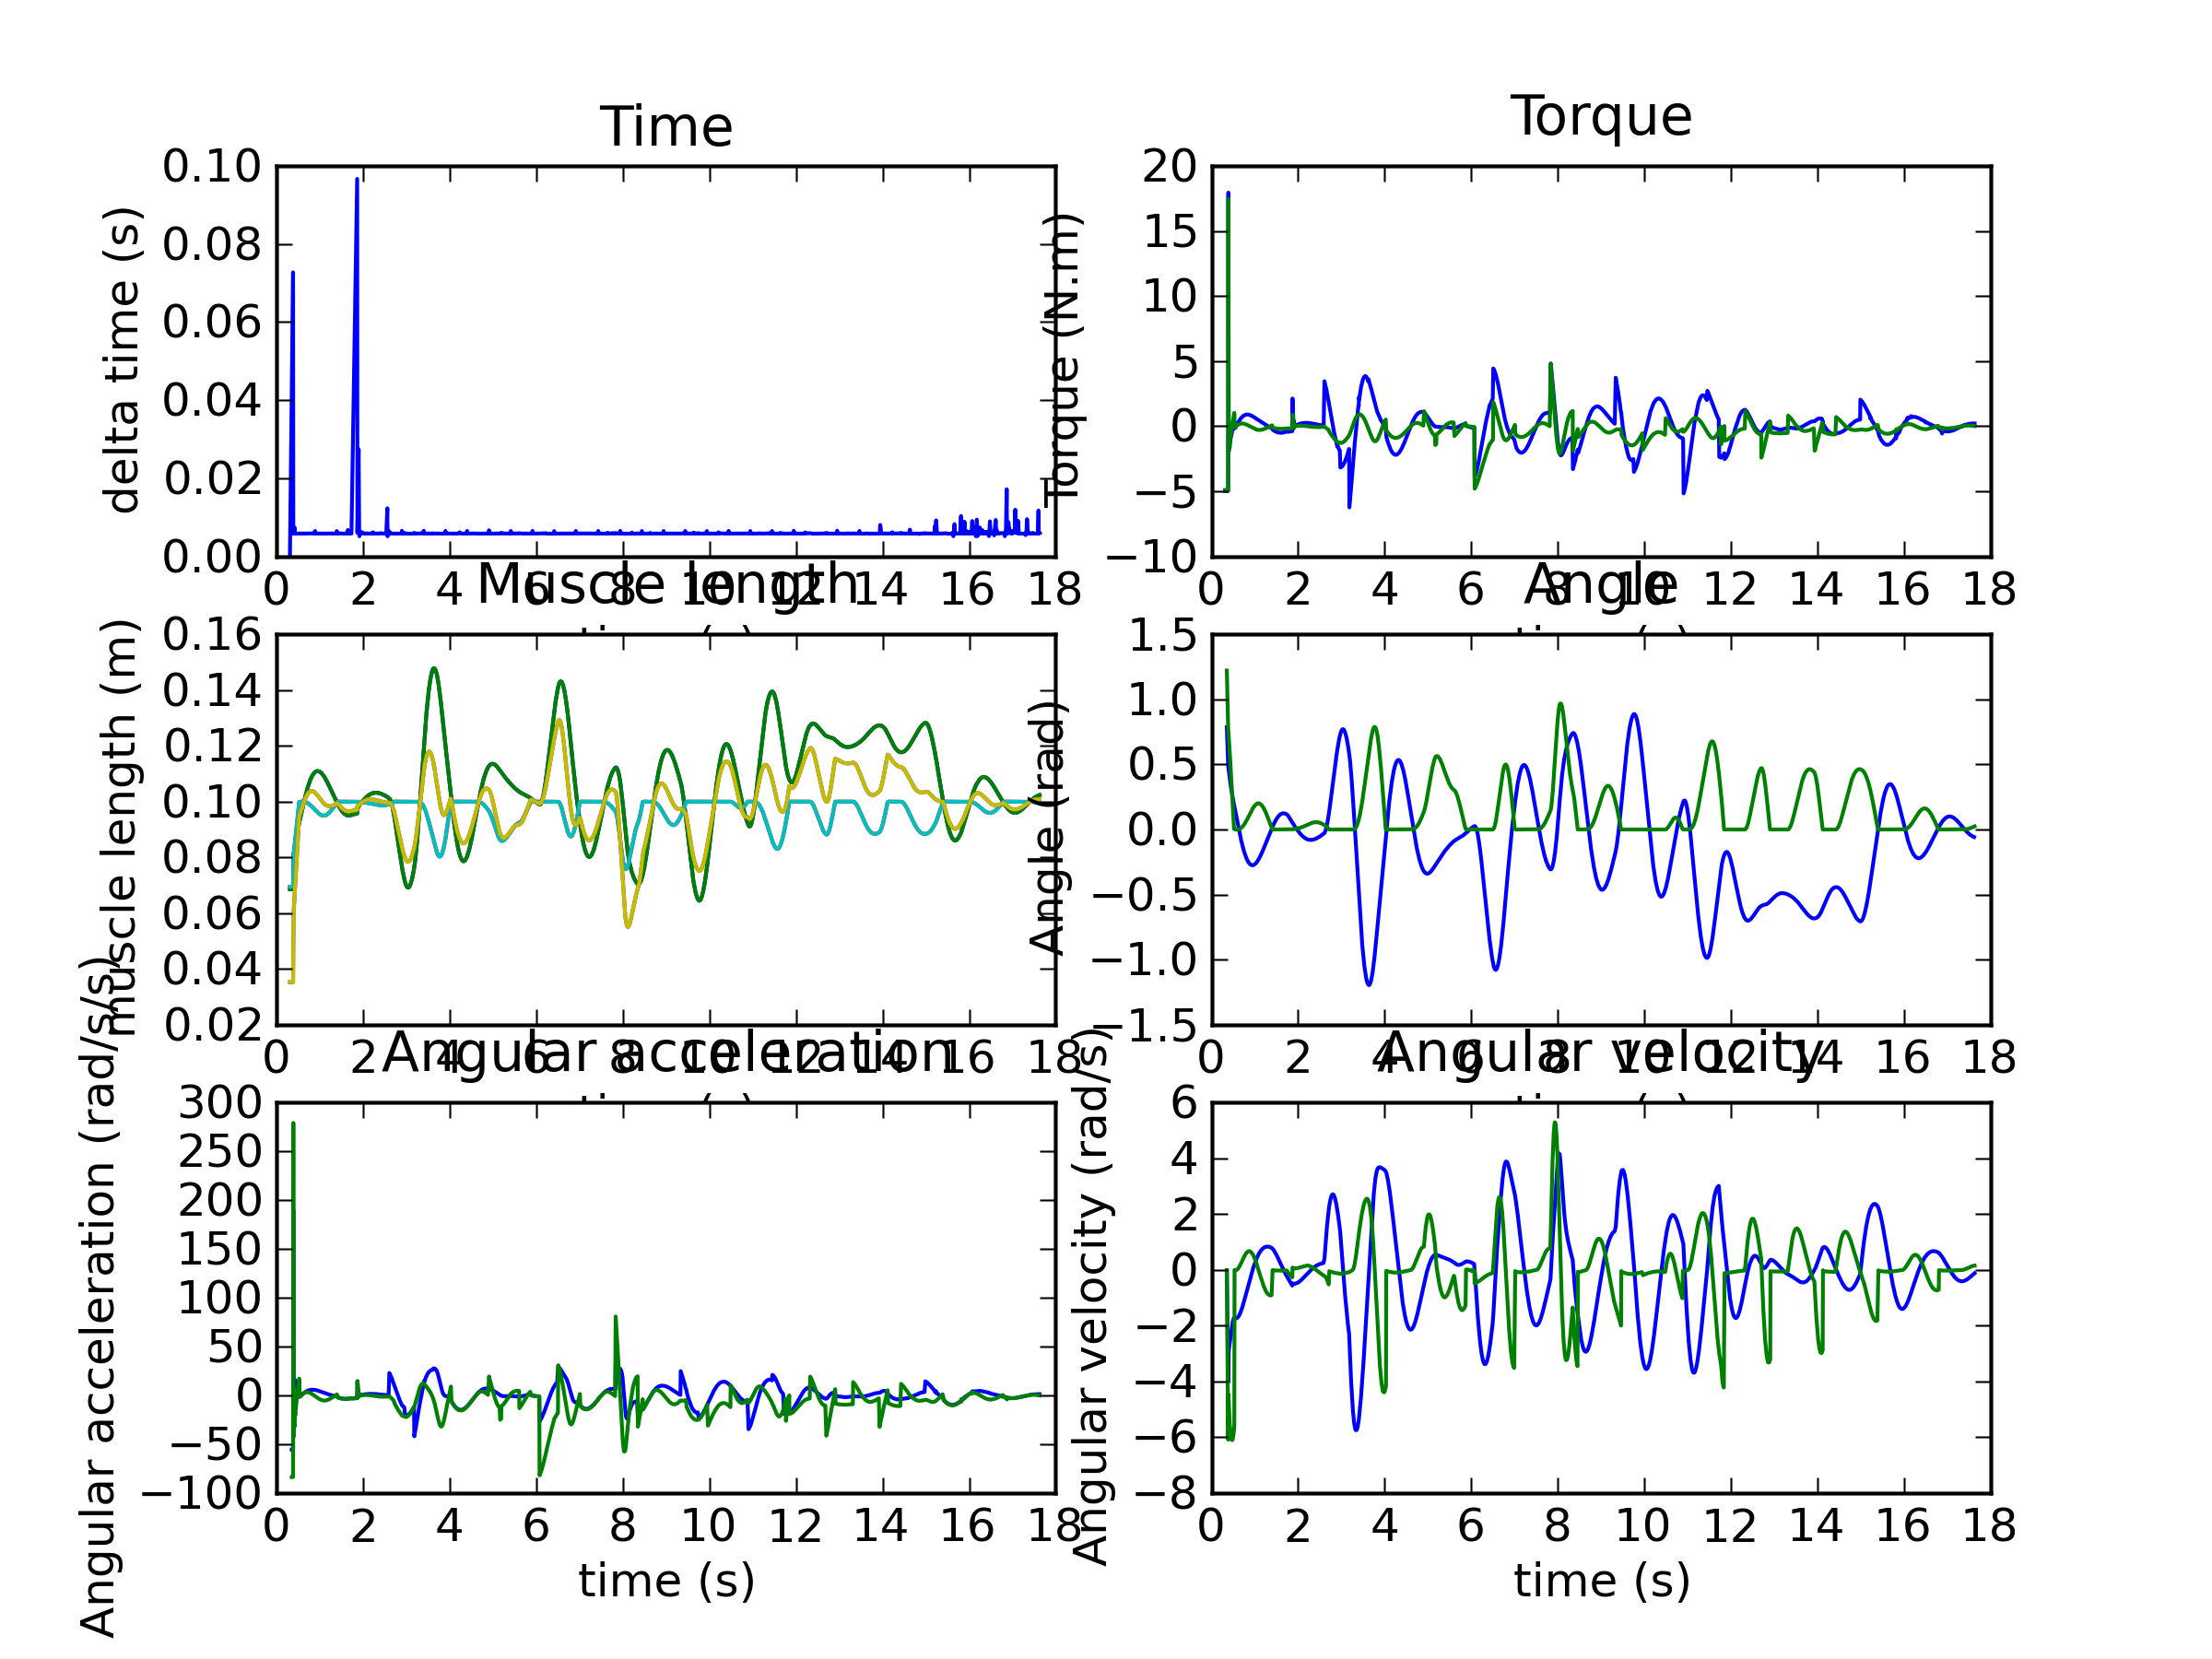
\includegraphics[width=.50\linewidth]{fig/pyarm2}}~~~
\end{figure}

\paragraph{}
Le simulateur est composé de 5 modules :
\begin{itemize}
    \item Filtre sur signal d'entrée
    \item Modèle de bras
    \begin{itemize}
        \item Cinématique
        \item Dynamique
    \end{itemize}
    \item Modèle de muscles
    \begin{itemize}
        \item Cinématique
        \item Dynamique
    \end{itemize}
\end{itemize}

\paragraph{}
\begin{center}
        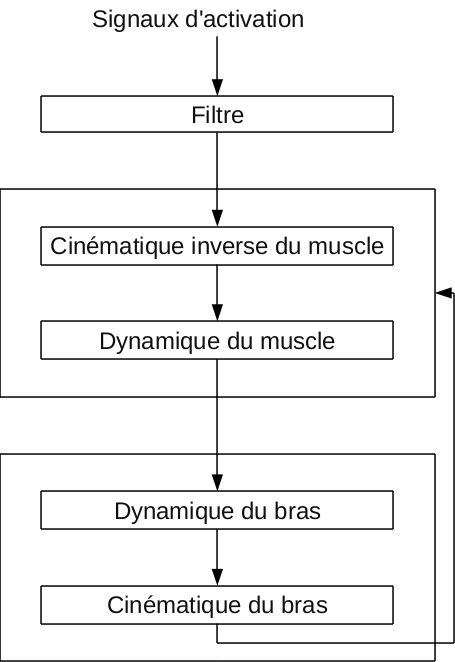
\includegraphics[width=.60\linewidth]{fig/modules}
\end{center}

%%%%%%%%%%%%%%%%%%%%%%%%%%%%%%%%%%%%%%%%%%%%%%%%%%%%%%%%%%%%%%%%%%%%%%%%%%%%%%%%

\section{Modèle du muscles}

\subsection{Mitrovic}

\begin{tabular}{lcl}
    $\tau$ & = & $-A^T t(l, \dot{l}, u)$ \\
    & & \\
    $t(l, \dot{l}, u)$        & = & $k(u) (l_r(u) - l) + b(u) \dot{l}$ \\
    & & \\
    $k(u)$    & = & $k_0 + k u$ \\
    $b(u)$    & = & $b_0 + b u$ \\
    $l_r(u)$  & = & $l_0 - r u$ \\
    & & \\
    $l$       & = & $l_m - A \theta $ \\
    $\dot{l}$ & = & $l_m - A \omega $ \\
\end{tabular}

\paragraph{}
\begin{tabular}{lcl}
    $\tau_i$ & = & Couple total exercé sur l'articulation $i$ \\
    $A$  & = & Matrice des bras de levier \\
    $t(l, \dot{l}, u)$  & = & Tension exercée par le muscle \\
    $k(u)$ & = & Raideur du muscle \\
    $b(u)$ & = & Viscosité du muscle \\
    $l_r(u)$ & = & Longueur du muscle au repos \\
    $l$ & = & Longueur du muscle \\
    $u$ & = & Signaux d'activation du muscle \\
    $k_0$ & = & Élasticité intrinsèque \\
    $b_0$ & = & Viscosité intrinsèque \\
    $l_0$ & = & Longueur du muscle au repos \\
    $k$ & = & Coefficient de variation de l'élasticité \\
    $b$ & = & Coefficient de variation de la viscosité \\
    $r$ & = & Coefficient de variation de la longueur au repos \\
    %$l_{0i}$ & = & Longueur du muscle au repos pour l'angle $\theta = 0$ \\
\end{tabular}

\begin{center}
        \includegraphics[width=.50\linewidth]{fig/moment_arm}
\end{center}

\subsection{Kambara}

\begin{tabular}{lcl}
    $\tau$ & = & $A^T T$ \\
    & & \\
    $T_i$                     & = & $K_i(\tilde{u}_i) (L_i - L_i^{rest}(\tilde{u}_i)) + B_i(\tilde{u}_i) \dot{L}_i$ \\
    & & \\
    $K_i(\tilde{u}_i)$        & = & $k_{0i} + k_{1i} \tilde{u}_i$ \\
    $B_i(\tilde{u}_i)$        & = & $b_{0i} + b_{1i} \tilde{u}_i$ \\
    $L_i^{rest}(\tilde{u}_i)$ & = & $ l_{0i}^{rest} - l_{1i}^{rest} \tilde{u}_i$ \\
    & & \\
    $L_i$ & = & $l_{0i} - \sum_{j=1}^2 A_{i,j} \theta_j $ \\
\end{tabular}

\paragraph{}
\begin{tabular}{lcl}
    $\tau_i$ & = & Couple total exercé sur l'articulation $i$ \\
    $A$  & = & Matrice des bras de levier \\
    $T_i$  & = & Tension exercée par le muscle $i$ \\
    $K_i(\tilde{u}_i)$ & = & Raideur du muscle $i$ \\
    $B_i(\tilde{u}_i)$ & = & Viscosité du muscle $i$ \\
    $L_i^{rest}(\tilde{u}_i)$ & = & Longueur du muscle $i$ au repos \\
    $L_i$ & = & Longueur du muscle $i$ \\
    $\tilde{u}_i$ & = & Signaux d'activation filtrés du muscle $i$ \\
    $k_{0i}$ & = & Élasticité intrinsèque \\
    $b_{0i}$ & = & Viscosité intrinsèque \\
    $l^{rest}_{0i}$ & = & Longueur du muscle $i$ au repos \\
    $k_{1i}$ & = & Coefficient de variation de l'élasticité \\
    $b_{1i}$ & = & Coefficient de variation de la viscosité \\
    $l^{rest}_{1i}$ & = & Coefficient de variation de la longueur au repos \\
    $l_{0i}$ & = & Longueur du muscle $i$ au repos pour l'angle $\theta = 0$ \\
\end{tabular}

\subsection{Weiwei}

\begin{center}
        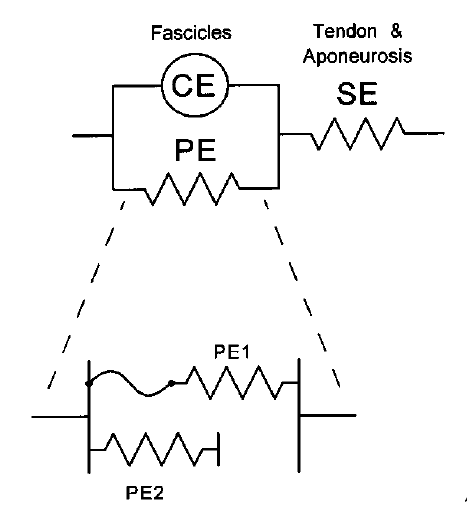
\includegraphics[width=.40\linewidth]{fig/brown}
\end{center}

\begin{tabular}{lcl}
    $CE$  & = & éléments contractiles \\
    $SE$  & = & élasticité des tendons (ignorée) \\
    $PE$  & = & élasticité du muscle \\
    $PE1$ & = & résistance à l'étirement du muscle passif \\
    $PE2$ & = & résistance à la compression du muscle actif \\
\end{tabular}


%%%%%%%%%%%%%%%%%%%%%%%%%%%%%%%%%%%%%%%%%%%%%%%%%%%%%%%%%%%%%%%%%%%%%%%%%%%%%%%%

\section{Modèle du bras}

%%%%%%%%

\subsection{Cas général}

\subsubsection{Dynamique inverse}
$\tau = M(\theta)\alpha + C(\theta, \omega) + b(\omega) + g(\theta) $ (1)

\subsubsection{Dynamique}
(1) $\Leftrightarrow \alpha = M(\theta)^{-1} + (\tau - C(\theta, \omega) - b(\omega) - g(\theta)) $

\subsubsection{Légende}
\begin{tabular}{lcl}
    $M$      & = & matrice des moments d'inertie \\ % TODO
    $C$      & = & force de Coriolis et force centripète \\
    $b$      & = & force de viscosité et de friction \\ % TODO
    $g$      & = & force de gravité \\
    $\tau$   & = & couple total exercé sur les articulations ($N.m$) \\
    $\alpha$ & = & accélération angulaire ($rd.s^{-2}$) \\
    $\omega$ & = & vitesse angulaire ($rd.s^{-1}$) \\
    $\theta$ & = & angle ($rd$) \\
\end{tabular}

%%%%%%%%

\subsection{Mitrovic}

\subsubsection{Dynamique inverse}
$\tau = M(\theta)\alpha + C(\theta, \omega) \omega $ (2)

\subsubsection{Dynamique}
(2) $\Leftrightarrow \alpha = M(\theta)^{-1} + (\tau - C(\theta, \omega) \omega) $

%%%%%%%%

\subsection{Kambara}

\subsubsection{Dynamique inverse}
$
\begin{pmatrix}
    \tau_1 \\
    \tau_2 \\
\end{pmatrix}
=
\begin{pmatrix}
    M_{11}\alpha_1 + M_{12}\alpha_2 + h_{122}\omega_2^2 + 2h_{112}\omega_1\omega_2 + g_1 \\
    M_{21}\alpha_1 + M_{22}\alpha_2 + h_{211}\omega_1^2 + g_2 \\
\end{pmatrix}
(3)$

\paragraph{}
\begin{tabular}{lcl}
    $M_{11}$ & = & $I_1 + I_2 + m_2(l_1^2 + 2 l_1 l_{g2}\cos\theta_2$) \\
    $M_{12}$ & = & $I_2 + m_2l_1l_{g2}\cos\theta_2$ \\
    $M_{21}$ & = & $I_2 + m_2l_1l_{g2}\cos\theta_2$ \\
    $M_{22}$ & = & $I_2$ \\
    $h_{122}$ & = & $-m_2 l_1 l_{g2} \sin\theta_2$ \\
    $h_{112}$ & = & $-m_2 l_1 l_{g2} \sin\theta_2$ \\
    $h_{211}$ & = & $m_2 l_1 l_{g2} \sin\theta_2$ \\
    $g_1$ & = & $m_1 \hat{g} l_{g1} \cos\theta_1 + m_2 \hat{g} (l_1 \cos\theta_1 + l_{g2} \cos(\theta_1 + \theta_2))$ \\
    $g_2$ & = & $m_2 \hat{g} l_{g2} \cos(\theta_1 + \theta_2))$ \\
    & & \\
    $m_j$ & = & masse du membre \\
    $l_j$ & = & longueur du membre \\
    $l_{gj}$ & = & distance séparant le centre de masse de l'articulation \\
    $I_{j}$ & = & moment d'inertie \\
    $\hat{g}$ & = & champ de pesanteur \\
\end{tabular}

\paragraph{}
\begin{tabular}{lcl}
    (3) & $\Leftrightarrow$ & $\tau = M(\theta)\alpha + C(\theta, \omega) \omega + g$ \\
\end{tabular}

\subsubsection{Dynamique}
(3) $\Leftrightarrow \alpha = M(\theta)^{-1} + (\tau - C(\theta, \omega) \omega - g) $

%%%%%%%%

\subsection{Weiwei}

\subsubsection{Dynamique inverse}
$\tau = M(\theta)\alpha + C(\theta, \omega) + B\omega $ (4)

\paragraph{}
\begin{tabular}{lcl}
    $M$ & = &
    $
    \begin{pmatrix}
        d1 + 2 d_2 \cos\theta_2  & d_3 + d_2 \cos \theta_2 \\
        d_3 + d_2 \cos\theta_2 & d_3 \\
    \end{pmatrix}
    $ \\

    $C$ & = &
    $
    \begin{pmatrix}
        -\omega_2 (2 \omega_1 + \omega_2) \\
        \omega_1^2 \\
    \end{pmatrix}
    d_2 \sin\theta_2
    $\\

    $B$ & = &
    $
    \begin{pmatrix}
        0.05  & 0.025 \\
        0.025 & 0.05 \\
    \end{pmatrix}
    $
\end{tabular}

\paragraph{}
\begin{tabular}{lcl}
    $d_1$ & = & $I_1 + I_2 + m_2 l_1^2$ \\
    $d_2$ & = & $m_2 l_1 s_2$ \\
    $d_3$ & = & $I_2$ \\
\end{tabular}

\paragraph{}
\begin{tabular}{lcl}
    $m_j$ & = & masse du membre \\
    $l_j$ & = & longueur du membre \\
    $s_{j}$ & = & distance séparant le centre de masse de l'articulation \\
    $I_{j}$ & = & moment d'inertie \\
\end{tabular}

\subsubsection{Dynamique}
(4) $\Leftrightarrow \alpha = M(\theta)^{-1} + (\tau - C(\theta, \omega) - B\omega) $

\subsection{Résumé}
\begin{tabular}{|c|l|}
    \hline
    Mitrovic  & $\alpha = M(\theta)^{-1} + (\tau - C(\theta, \omega) \omega)$ \\
    \hline
    Kambara  & $\alpha = M(\theta)^{-1} + (\tau - C(\theta, \omega) \omega - g)$ \\
    \hline
    Weiwei  & $\alpha = M(\theta)^{-1} + (\tau - C(\theta, \omega) - B\omega)$ \\
    \hline
\end{tabular}

%%%%%%%%%%%%%%%%%%%%%%%%%%%%%%%%%%%%%%%%%%%%%%%%%%%%%%%%%%%%%%%%%%%%%%%%%%%%%%%%

\section{Bibliographie}

\begin{center}
        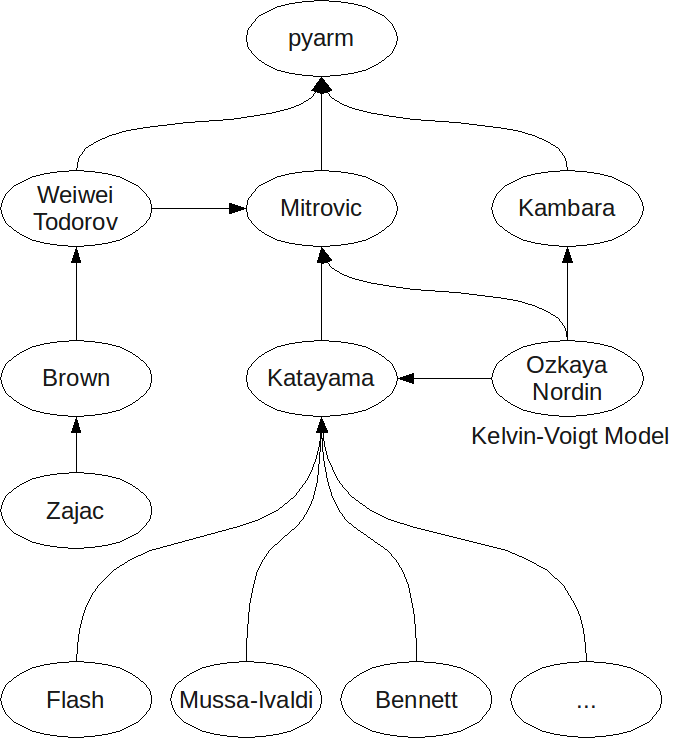
\includegraphics[width=.80\linewidth]{fig/bib}
\end{center}

\end{document}
